\documentclass[twoside]{book}

% Packages required by doxygen
\usepackage{fixltx2e}
\usepackage{calc}
\usepackage{doxygen}
\usepackage[export]{adjustbox} % also loads graphicx
\usepackage{graphicx}
\usepackage[utf8]{inputenc}
\usepackage{makeidx}
\usepackage{multicol}
\usepackage{multirow}
\PassOptionsToPackage{warn}{textcomp}
\usepackage{textcomp}
\usepackage[nointegrals]{wasysym}
\usepackage[table]{xcolor}

% Font selection
\usepackage[T1]{fontenc}
\usepackage[scaled=.90]{helvet}
\usepackage{courier}
\usepackage{amssymb}
\usepackage{sectsty}
\renewcommand{\familydefault}{\sfdefault}
\allsectionsfont{%
  \fontseries{bc}\selectfont%
  \color{darkgray}%
}
\renewcommand{\DoxyLabelFont}{%
  \fontseries{bc}\selectfont%
  \color{darkgray}%
}
\newcommand{\+}{\discretionary{\mbox{\scriptsize$\hookleftarrow$}}{}{}}

% Page & text layout
\usepackage{geometry}
\geometry{%
  a4paper,%
  top=2.5cm,%
  bottom=2.5cm,%
  left=2.5cm,%
  right=2.5cm%
}
\tolerance=750
\hfuzz=15pt
\hbadness=750
\setlength{\emergencystretch}{15pt}
\setlength{\parindent}{0cm}
\setlength{\parskip}{3ex plus 2ex minus 2ex}
\makeatletter
\renewcommand{\paragraph}{%
  \@startsection{paragraph}{4}{0ex}{-1.0ex}{1.0ex}{%
    \normalfont\normalsize\bfseries\SS@parafont%
  }%
}
\renewcommand{\subparagraph}{%
  \@startsection{subparagraph}{5}{0ex}{-1.0ex}{1.0ex}{%
    \normalfont\normalsize\bfseries\SS@subparafont%
  }%
}
\makeatother

% Headers & footers
\usepackage{fancyhdr}
\pagestyle{fancyplain}
\fancyhead[LE]{\fancyplain{}{\bfseries\thepage}}
\fancyhead[CE]{\fancyplain{}{}}
\fancyhead[RE]{\fancyplain{}{\bfseries\leftmark}}
\fancyhead[LO]{\fancyplain{}{\bfseries\rightmark}}
\fancyhead[CO]{\fancyplain{}{}}
\fancyhead[RO]{\fancyplain{}{\bfseries\thepage}}
\fancyfoot[LE]{\fancyplain{}{}}
\fancyfoot[CE]{\fancyplain{}{}}
\fancyfoot[RE]{\fancyplain{}{\bfseries\scriptsize Generated by Doxygen }}
\fancyfoot[LO]{\fancyplain{}{\bfseries\scriptsize Generated by Doxygen }}
\fancyfoot[CO]{\fancyplain{}{}}
\fancyfoot[RO]{\fancyplain{}{}}
\renewcommand{\footrulewidth}{0.4pt}
\renewcommand{\chaptermark}[1]{%
  \markboth{#1}{}%
}
\renewcommand{\sectionmark}[1]{%
  \markright{\thesection\ #1}%
}

% Indices & bibliography
\usepackage{natbib}
\usepackage[titles]{tocloft}
\setcounter{tocdepth}{3}
\setcounter{secnumdepth}{5}
\makeindex

% Hyperlinks (required, but should be loaded last)
\usepackage{ifpdf}
\ifpdf
  \usepackage[pdftex,pagebackref=true]{hyperref}
\else
  \usepackage[ps2pdf,pagebackref=true]{hyperref}
\fi
\hypersetup{%
  colorlinks=true,%
  linkcolor=blue,%
  citecolor=blue,%
  unicode%
}

% Custom commands
\newcommand{\clearemptydoublepage}{%
  \newpage{\pagestyle{empty}\cleardoublepage}%
}

\usepackage{caption}
\captionsetup{labelsep=space,justification=centering,font={bf},singlelinecheck=off,skip=4pt,position=top}

%===== C O N T E N T S =====

\begin{document}

% Titlepage & ToC
\hypersetup{pageanchor=false,
             bookmarksnumbered=true,
             pdfencoding=unicode
            }
\pagenumbering{roman}
\begin{titlepage}
\vspace*{7cm}
\begin{center}%
{\Large Proto\+Test }\\
\vspace*{1cm}
{\large Generated by Doxygen 1.8.11}\\
\end{center}
\end{titlepage}
\clearemptydoublepage
\tableofcontents
\clearemptydoublepage
\pagenumbering{arabic}
\hypersetup{pageanchor=true}

%--- Begin generated contents ---
\chapter{Hierarchical Index}
\section{Class Hierarchy}
This inheritance list is sorted roughly, but not completely, alphabetically\+:\begin{DoxyCompactList}
\item \contentsline{section}{Proto\+Handler}{\pageref{class_proto_handler}}{}
\item \contentsline{section}{Services}{\pageref{class_services}}{}
\begin{DoxyCompactList}
\item \contentsline{section}{Service\+Implementation}{\pageref{class_service_implementation}}{}
\item \contentsline{section}{Service\+Implementation}{\pageref{class_service_implementation}}{}
\end{DoxyCompactList}
\item \contentsline{section}{Z\+M\+Q\+Handler}{\pageref{class_z_m_q_handler}}{}
\end{DoxyCompactList}

\chapter{Class Index}
\section{Class List}
Here are the classes, structs, unions and interfaces with brief descriptions\+:\begin{DoxyCompactList}
\item\contentsline{section}{\hyperlink{class_proto_handler}{Proto\+Handler} }{\pageref{class_proto_handler}}{}
\item\contentsline{section}{\hyperlink{class_service_implementation}{Service\+Implementation} }{\pageref{class_service_implementation}}{}
\item\contentsline{section}{\hyperlink{class_services}{Services} }{\pageref{class_services}}{}
\item\contentsline{section}{\hyperlink{class_z_m_q_handler}{Z\+M\+Q\+Handler} }{\pageref{class_z_m_q_handler}}{}
\end{DoxyCompactList}

\chapter{Class Documentation}
\hypertarget{class_proto_handler}{}\section{Proto\+Handler Class Reference}
\label{class_proto_handler}\index{Proto\+Handler@{Proto\+Handler}}
\subsection*{Public Member Functions}
\begin{DoxyCompactItemize}
\item 
void {\bfseries proto\+Method} (std\+::string \&message, std\+::string \&message\+Header)\hypertarget{class_proto_handler_a4fcfc152c4ec985003aed0e4a4354d73}{}\label{class_proto_handler_a4fcfc152c4ec985003aed0e4a4354d73}

\item 
void {\bfseries proto\+Print} (std\+::string \&message)\hypertarget{class_proto_handler_aab7c34f1297a4e7683ef2fd9f597ae0a}{}\label{class_proto_handler_aab7c34f1297a4e7683ef2fd9f597ae0a}

\item 
void {\bfseries proto\+Method} (std\+::string \&message, std\+::string \&message\+Header)\hypertarget{class_proto_handler_a4fcfc152c4ec985003aed0e4a4354d73}{}\label{class_proto_handler_a4fcfc152c4ec985003aed0e4a4354d73}

\end{DoxyCompactItemize}


The documentation for this class was generated from the following files\+:\begin{DoxyCompactItemize}
\item 
src/client/proto\+Handler\+Client.\+hpp\item 
src/server/proto\+Handler\+Server.\+hpp\item 
src/client/proto\+Handler\+Client.\+cpp\item 
src/server/proto\+Handler\+Server.\+cpp\end{DoxyCompactItemize}

\hypertarget{class_service_implementation}{}\section{Service\+Implementation Class Reference}
\label{class_service_implementation}\index{Service\+Implementation@{Service\+Implementation}}
Inheritance diagram for Service\+Implementation\+:\begin{figure}[H]
\begin{center}
\leavevmode
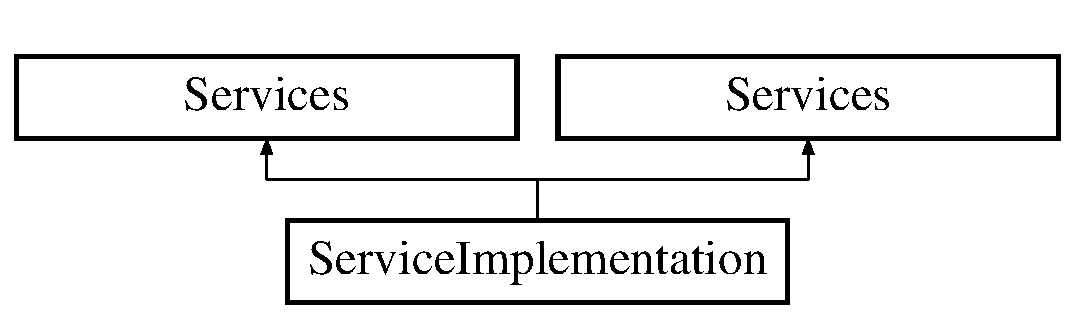
\includegraphics[height=2.000000cm]{class_service_implementation}
\end{center}
\end{figure}
\subsection*{Public Member Functions}
\begin{DoxyCompactItemize}
\item 
void {\bfseries get\+Nav} ()\hypertarget{class_service_implementation_a8bdcc77581d536e52dce63004f96d6c5}{}\label{class_service_implementation_a8bdcc77581d536e52dce63004f96d6c5}

\item 
void {\bfseries get\+Nav} ()\hypertarget{class_service_implementation_a8bdcc77581d536e52dce63004f96d6c5}{}\label{class_service_implementation_a8bdcc77581d536e52dce63004f96d6c5}

\end{DoxyCompactItemize}


The documentation for this class was generated from the following files\+:\begin{DoxyCompactItemize}
\item 
src/client/services\+Implementation.\+cpp\item 
src/server/server\+Implementation.\+cpp\end{DoxyCompactItemize}

\hypertarget{class_services}{}\section{Services Class Reference}
\label{class_services}\index{Services@{Services}}
Inheritance diagram for Services\+:\begin{figure}[H]
\begin{center}
\leavevmode
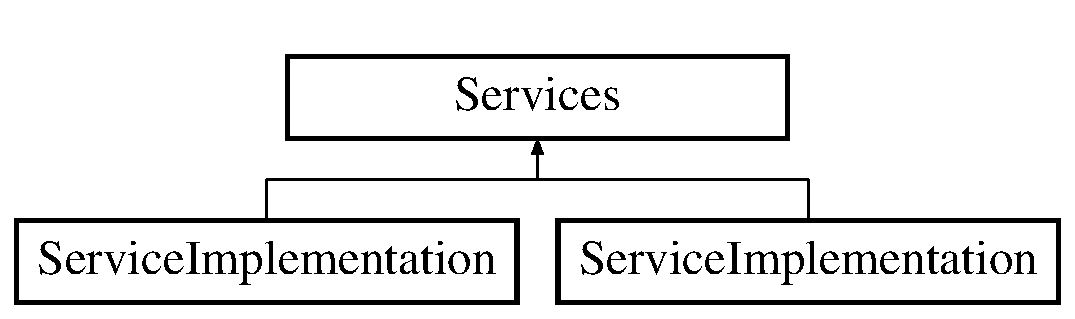
\includegraphics[height=2.000000cm]{class_services}
\end{center}
\end{figure}
\subsection*{Public Member Functions}
\begin{DoxyCompactItemize}
\item 
virtual void {\bfseries get\+Nav} ()=0\hypertarget{class_services_a003919830789e1d96441e6f8c00929e0}{}\label{class_services_a003919830789e1d96441e6f8c00929e0}

\item 
virtual void {\bfseries get\+Nav} ()=0\hypertarget{class_services_a003919830789e1d96441e6f8c00929e0}{}\label{class_services_a003919830789e1d96441e6f8c00929e0}

\item 
virtual void {\bfseries get\+Nav} ()=0\hypertarget{class_services_a003919830789e1d96441e6f8c00929e0}{}\label{class_services_a003919830789e1d96441e6f8c00929e0}

\item 
virtual void {\bfseries get\+Nav} ()=0\hypertarget{class_services_a003919830789e1d96441e6f8c00929e0}{}\label{class_services_a003919830789e1d96441e6f8c00929e0}

\end{DoxyCompactItemize}


The documentation for this class was generated from the following files\+:\begin{DoxyCompactItemize}
\item 
src/client/client\+Interface.\+hpp\item 
src/client/services\+Interface.\+cpp\item 
src/client/services\+Interface.\+hpp\item 
src/server/server\+Interface.\+hpp\end{DoxyCompactItemize}

\hypertarget{class_z_m_q_handler}{}\section{Z\+M\+Q\+Handler Class Reference}
\label{class_z_m_q_handler}\index{Z\+M\+Q\+Handler@{Z\+M\+Q\+Handler}}
\subsection*{Public Member Functions}
\begin{DoxyCompactItemize}
\item 
void {\bfseries zmq\+Method} (std\+::string \&message, std\+::string \&message\+Header)\hypertarget{class_z_m_q_handler_a2b25bb9a6b699f34b46e8ac9a720920f}{}\label{class_z_m_q_handler_a2b25bb9a6b699f34b46e8ac9a720920f}

\item 
void {\bfseries zmq\+Read\+Method} (std\+::string \&message, std\+::string \&message\+Header)\hypertarget{class_z_m_q_handler_ac490adce32e43430d97df9d182a9fafa}{}\label{class_z_m_q_handler_ac490adce32e43430d97df9d182a9fafa}

\item 
void {\bfseries zmq\+Reply\+Method} (std\+::string \&message)\hypertarget{class_z_m_q_handler_a3f80778a54859fdb870e053e8ed459f3}{}\label{class_z_m_q_handler_a3f80778a54859fdb870e053e8ed459f3}

\end{DoxyCompactItemize}


The documentation for this class was generated from the following files\+:\begin{DoxyCompactItemize}
\item 
src/client/Z\+M\+Q\+Handler\+Client.\+hpp\item 
src/server/Z\+M\+Q\+Handler\+Server.\+hpp\item 
src/client/Z\+M\+Q\+Handler\+Client.\+cpp\item 
src/server/Z\+M\+Q\+Handler\+Server.\+cpp\end{DoxyCompactItemize}

%--- End generated contents ---

% Index
\backmatter
\newpage
\phantomsection
\clearemptydoublepage
\addcontentsline{toc}{chapter}{Index}
\printindex

\end{document}
